%% LyX 2.3.4.2 created this file.  For more info, see http://www.lyx.org/.
%% Do not edit unless you really know what you are doing.
\documentclass[english,dvipsnames,aspectratio=169]{beamer}
\usepackage{mathptmx}
\usepackage{eulervm}
\usepackage[T1]{fontenc}
\usepackage[latin9]{inputenc}
\usepackage{babel}
\usepackage{amstext}
\usepackage{amssymb}
\usepackage{graphicx}
\usepackage{ifthen}
\usepackage{xcolor}
\usepackage{xspace}
\usepackage{tikz}
\usetikzlibrary{tikzmark}
\usetikzlibrary{calc}
\usepackage{pgfplots}
%\pgfplotsset{compat=1.17}
\usepackage{booktabs}
\usepackage{xpatch}

\xpatchcmd{\itemize}
  {\def\makelabel}
  {\ifnum\@itemdepth=1\relax
     \setlength\itemsep{2ex}% separation for first level
   \else
     \ifnum\@itemdepth=2\relax
       \setlength\itemsep{1ex}% separation for second level
     \else
       \ifnum\@itemdepth=3\relax
         \setlength\itemsep{0.5ex}% separation for third level
   \fi\fi\fi\def\makelabel
  }
 {}
 {}

\ifx\hypersetup\undefined
  \AtBeginDocument{%
    \hypersetup{unicode=true,pdfusetitle,
 bookmarks=true,bookmarksnumbered=false,bookmarksopen=false,
 breaklinks=false,pdfborder={0 0 0},pdfborderstyle={},backref=false,colorlinks=true,
 allcolors=NYUPurple,urlcolor=LightPurple}
  }
\else
  \hypersetup{unicode=true,pdfusetitle,
 bookmarks=true,bookmarksnumbered=false,bookmarksopen=false,
 breaklinks=false,pdfborder={0 0 0},pdfborderstyle={},backref=false,colorlinks=true,
 allcolors=NYUPurple,urlcolor=LightPurple}
\fi

\makeatletter

%%%%%%%%%%%%%%%%%%%%%%%%%%%%%% LyX specific LaTeX commands.
%% Because html converters don't know tabularnewline
\providecommand{\tabularnewline}{\\}

%%%%%%%%%%%%%%%%%%%%%%%%%%%%%% Textclass specific LaTeX commands.
% this default might be overridden by plain title style
\newcommand\makebeamertitle{\frame{\maketitle}}%
% (ERT) argument for the TOC
\AtBeginDocument{%
  \let\origtableofcontents=\tableofcontents
  \def\tableofcontents{\@ifnextchar[{\origtableofcontents}{\gobbletableofcontents}}
  \def\gobbletableofcontents#1{\origtableofcontents}
}

%%%%%%%%%%%%%%%%%%%%%%%%%%%%%% User specified LaTeX commands.
\usetheme{CambridgeUS} 
\beamertemplatenavigationsymbolsempty


% Set Color ==============================
\definecolor{NYUPurple}{RGB}{87,6,140}
\definecolor{LightPurple}{RGB}{165,11,255}


\setbeamercolor{title}{fg=NYUPurple}
\setbeamercolor{frametitle}{fg=NYUPurple}

\setbeamercolor{background canvas}{fg=NYUPurple, bg=white}
\setbeamercolor{background}{fg=black, bg=NYUPurple}

\setbeamercolor{palette primary}{fg=black, bg=gray!30!white}
\setbeamercolor{palette secondary}{fg=black, bg=gray!20!white}
\setbeamercolor{palette tertiary}{fg=gray!20!white, bg=NYUPurple}

\setbeamertemplate{headline}{}
\setbeamerfont{itemize/enumerate body}{}
\setbeamerfont{itemize/enumerate subbody}{size=\normalsize}

\setbeamercolor{parttitle}{fg=NYUPurple}
\setbeamercolor{sectiontitle}{fg=NYUPurple}
\setbeamercolor{sectionname}{fg=NYUPurple}
\setbeamercolor{section page}{fg=NYUPurple}
%\setbeamercolor{description item}{fg=NYUPurple}
%\setbeamercolor{block title}{fg=NYUPurple}

\setbeamertemplate{blocks}[rounded][shadow=false]
\setbeamercolor{block body}{bg=normal text.bg!90!NYUPurple}
\setbeamercolor{block title}{bg=NYUPurple!30, fg=NYUPurple}



\AtBeginSection[]{
  \begin{frame}
  \vfill
  \centering
\setbeamercolor{section title}{fg=NYUPurple}
 \begin{beamercolorbox}[sep=8pt,center,shadow=true,rounded=true]{title}
    \usebeamerfont{title}\usebeamercolor[fg]{title}\insertsectionhead\par%
  \end{beamercolorbox}
  \vfill
  \end{frame}
}

\makeatother

\setlength{\parskip}{\medskipamount} 

\input ../macros

\begin{document}
\input ../rosenberg-macros

\title[DS-GA 1003]{Gradient Descent, Stochastic Gradient Descent and Loss Functions\\\vspace{0.5in}\small{Based on David Rosenberg and He He's materials}}
\author{Tal Linzen}

\date{Feb 1, 2022}
\institute{CDS, NYU}

\makebeamertitle
\mode<article>{Just in article version}

\section{Review: ERM}
\begin{frame}{Our Setup from Statistical Learning Theory}
\begin{block}{The Spaces}
\begin{columns}[t]

\column{.3\textwidth}
\begin{itemize}
\item $\cx$: input space
\end{itemize}

\column{.3\textwidth}
\begin{itemize}
\item $\cy$: outcome space 
\end{itemize}

\column{.3\textwidth}
\begin{itemize}
\item $\ca$: action space
\end{itemize}
\end{columns}

\end{block}

\begin{block}{Prediction Function (or ``decision function'')}

A \textbf{prediction function }(or \textbf{decision function}) gets
input $x\in\cx$ and produces an action $a\in\ca$ :

\[
\begin{matrix}f: & \cx & \rightarrow & \ca\\
 & x & \mapsto & f(x)
\end{matrix}
\]
\end{block}
\pause
\begin{block}{Loss Function}

A \textbf{loss function} evaluates an action in the context of the
outcome $y$.

\[
\begin{matrix}\loss: & \ca\times\cy & \rightarrow & \reals\\
& (a,y) & \mapsto & \loss(a,y)
\end{matrix}
\]

\end{block}
\end{frame}
%
\begin{frame}{Risk and the Bayes Prediction Function }
\begin{definition}
The \textbf{risk}\emph{ }of a prediction function $f:\cx\to\ca$ is
\[
R(f)=\ex\loss(f(x),y).
\]
In words, it's the \textbf{expected loss} of $f$ on a new example
$(x,y)$ drawn randomly from $P_{\cx\times\cy}$.
\end{definition}

\pause
\begin{definition}
A \textbf{Bayes prediction function} $\minimizer f:\cx\to\ca$ is
a function that achieves the \emph{minimal risk} among all possible
functions: 
\[
\minimizer f\in\argmin_{f}R(f),
\]
where the minimum is taken over all functions from $\cx$ to $\ca$. 
\end{definition}

\begin{itemize}
\item The risk of a Bayes prediction function is called the \textbf{Bayes
risk}.
\end{itemize}
\end{frame}
%
\begin{frame}{The Empirical Risk}

Let $\cd_{n}=\left((x_{1},y_{1}),\ldots,(x_{n},y_{n})\right)$ be
drawn i.i.d. from $\cp_{\cx\times\cy}$.
\begin{definition}
The \textbf{empirical risk}\emph{ }of $f:\cx\to\ca$ with respect
to $\cd_{n}$ is
\[
\hat{R}_{n}(f)=\frac{1}{n}\sum_{i=1}^{n}\loss(f(x_{i}),y_{i}).
\]
\end{definition}


\begin{itemize}
\item The \textbf{unconstrained} empirical risk minimizer can
overfit.

\begin{itemize}
\item i.e. if we minimize $\hat{R}_{n}(f)$ over\textbf{ all functions}, we
overfit. 
\end{itemize}
\end{itemize}
\end{frame}
%
\begin{frame}{Constrained Empirical Risk Minimization}
\begin{definition}
A \textbf{hypothesis space} $\cf$ is a set of functions mapping $\cx\to\ca$.
\begin{itemize}
\item This is the collection of prediction functions we are choosing from.
\end{itemize}
\end{definition}
\pause

\begin{itemize}
\item An \textbf{empirical risk minimizer }(ERM) in $\cf$ is 
\[
\hat{f}_{n}\in\argmin_{f\in\cf}\frac{1}{n}\sum_{i=1}^{n}\loss(f(x_{i}),y_{i}).
\]

\item From now on ``ERM'' always means ``constrained ERM''.
\item So we should always specify the hypothesis space when we're doing
ERM.
\end{itemize}
\end{frame}
%
\begin{frame}{Example: Linear Least Squares Regression}
\begin{block}{Setup}
\begin{itemize}
\pause
\item Input space $\cx=\reals^{d}$
\pause
\item Output space $\cy=\reals$
\pause
\item Action space $\cy=\reals$
\end{itemize}
\pause

\begin{itemize}
\item Loss: $\loss(\hat{y},y)=\left(y-\hat{y}\right)^{2}$
\pause
\item \textbf{Hypothesis space:} $\cf=\left\{ f:\reals^{d}\to\reals\mid f(x)=w^{T}x\,,\,w\in\reals^{d}\right\} $
\end{itemize}

\end{block}
\begin{itemize}
\item Given a data set $\cd_{n}=\left\{ (x_{1},y_{1}),\ldots,(x_{n},y_{n})\right\} $,
\begin{itemize}
\item Our goal is to find the ERM $\hat{f}\in\cf$. 
\end{itemize}
\end{itemize}
\end{frame}

\begin{frame}{Example: Linear Least Squares Regression}
\begin{block}{Objective Function: Empirical Risk}

We want to find the function in $\cf$, parametrized by $w\in\reals^{d}$, that minimizes the empirical risk: 
\[
\hat{R}_{n}(w)=\frac{1}{n}\sum_{i=1}^{n}\left(w^{T}x_{i}-y_{i}\right)^{2}
\]

\end{block}
\begin{itemize}
\item How do we solve this optimization problem?
    $$
        \min_{w\in\reals^d} \hat{R}_n(w) 
        $$
    \item (For OLS there's a closed form solution, but in general there isn't.)
\end{itemize}
\end{frame}

\section{Gradient Descent}

\begin{frame}{Unconstrained Optimization}
\begin{block}{Setting}

We assume that the objective function $f:\reals^{d}\to\reals$ is \emph{differentiable.}

We want to find 
\[
x^{*}=\arg\min_{x\in\reals^{d}}f(x)
\]
\end{block}
\end{frame}

\begin{frame}{The Gradient}
\begin{itemize}
\item Let $f:\reals^{d}\to\reals$ be differentiable at $x_{0}\in\reals^{d}$.
\end{itemize}

\begin{itemize}
\item The \textbf{gradient} of $f$  at the point $x_{0}$, denoted $\del_{x}f(x_{0})$,
    is the direction in which $f(x)$ \textbf{increases fastest},
if we start from $x_{0}$.
\end{itemize}
\begin{center}
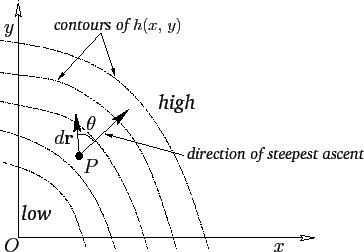
\includegraphics[height=0.4\textheight]{figures/two-dim-gradient}
\par\end{center}

\let\thefootnote\relax\footnotetext{\tiny{Figure A.111 from Newtonian Dynamics, by Richard Fitzpatrick.}}
\end{frame}

\begin{frame}{Gradient Descent}
\begin{itemize}
    \item To reach a local minimum as fast as possible, we want to go in the opposite direction from the gradient.
\end{itemize}
\pause
\begin{block}{Gradient Descent}
\begin{itemize}
\item Initialize $x \gets 0$.
\item Repeat:
\begin{itemize}
\item $x\gets x-\eta\del f(x)$
\end{itemize}
\item until the stopping criterion is satisfied.
\end{itemize}
\pause
\end{block}
    \begin{itemize}
        \item The ``step size'' $\eta$ is not the amount by which we update $x$!
    \end{itemize}
\end{frame}

\begin{frame}{Gradient Descent Path}
\begin{center}
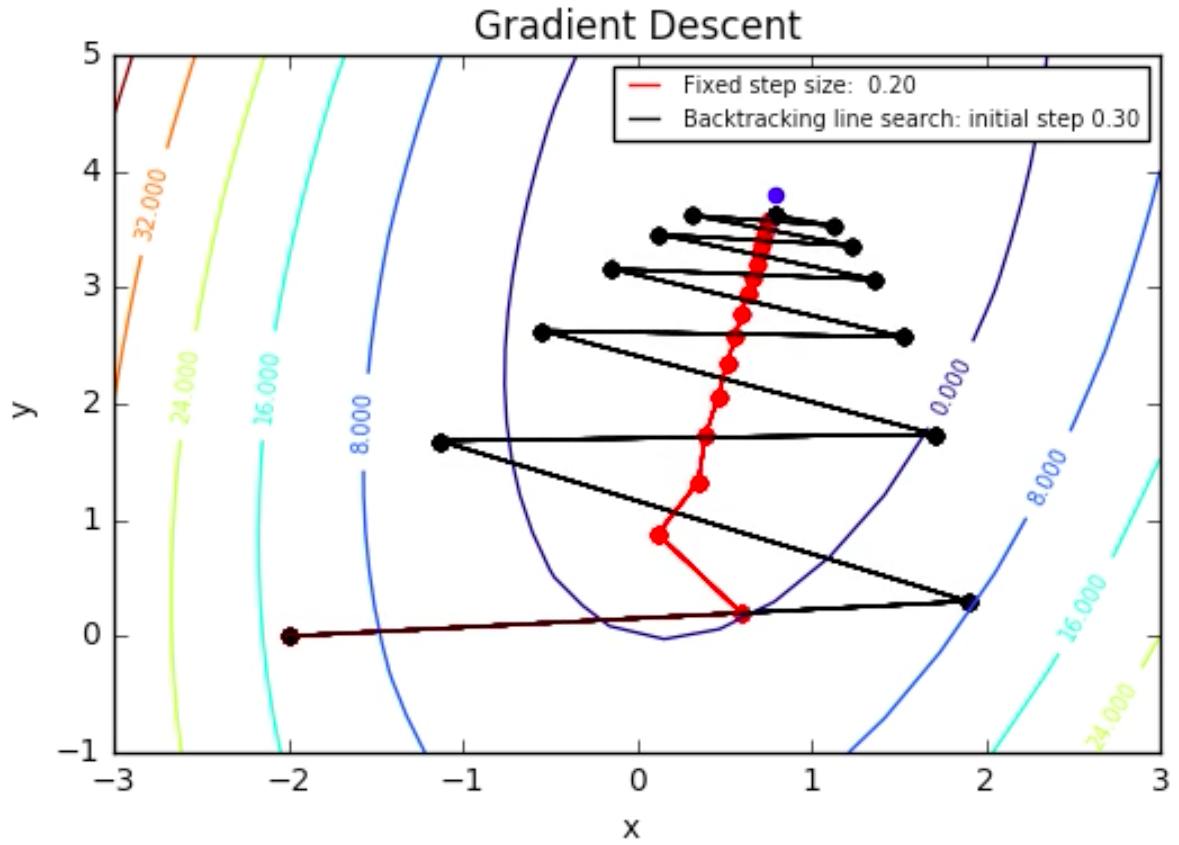
\includegraphics[height=0.8\textheight]{figures/vlad-GD-fixedAndBacktracking} 
\par\end{center}

\end{frame}

\begin{frame}{Gradient Descent: Step Size}
\begin{itemize}
\item A fixed step size will work, eventually, as long as it's small enough
(roughly --- details to come)
\begin{itemize}
\pause
\item If $\eta$ is too large, the optimization process might diverge
\pause
\item In practice, it often makes sense to try several fixed step sizes
\end{itemize}
\end{itemize}

\begin{itemize}
\item Intuition on when to take big steps and when to take small steps?
    \vspace{4em}
\end{itemize}
\end{frame}
%
\begin{frame}{Convergence Theorem for Fixed Step Size}
\begin{theorem}
Suppose $f:\reals^{d}\to\reals$ is convex and differentiable, and
$\del f$ is \textbf{Lipschitz continuous} with constant $L>0$, i.e.
\[
\|\del f(x)-\del f(x')\|\le L\|x-x'\|
\]
for any $x,x'\in\reals^{d}$. Then gradient descent with
fixed step size $\eta\le1/L$ \textbf{converges}. In particular,
\[
f(x^{(k)})-f(x^{*})\le\frac{\|x^{(0)}-x^{*}\|^{2}}{2\eta k}.
\]
\mode<article>{Proof sketch: Fit a quadratic at $x$ that's tangent to $f(x)$ and
has Lipschitz constant $L$. Taylor remainder theorem to show that
$f(x)$ is below quadratic. Jump to minimizer of quadratic.} 

\end{theorem}

This says that gradient descent is guaranteed to converge and that it converges with rate $O(1/k)$.
\end{frame}
%

\begin{frame}{Gradient Descent: When to Stop?}
\begin{itemize}
\item Wait until $\|\del f(x)\|_{2}\leq\eps$, for some $\eps$ of your
choosing.
\begin{itemize}
\item (Recall $\del f(x)=0$ at a local minimum.)
\end{itemize}
\end{itemize}
\pause

\begin{itemize}
\item Early stopping:
\begin{itemize}
\item evalute loss on validation data after each iteration;
\item stop when the loss does not improve (or gets worse).
\end{itemize}
\end{itemize}
\end{frame}


\section{Gradient Descent for Empirical Risk - Scaling Issues}

\begin{frame}{Quick recap: Gradient Descent for ERM}
\begin{itemize}
\item We have a hypothesis space of functions $\cf=\left\{ f_{w}:\cx\to\ca\mid w\in\reals^{d}\right\} $ 
\begin{itemize}
\item Parameterized by $w\in\reals^{d}$.
\end{itemize}

\item Finding an empirical risk minimizer entails finding a $w$ that minimizes
\[
\hat{R}_{n}(w)=\frac{1}{n}\sum_{i=1}^{n}\loss(f_{w}(x_{i}),y_{i})
\]
\item Suppose $\loss(f_{w}(x_{i}),y_{i})$ is differentiable as a function
of $w$.
\item Then we can do gradient descent on $\hat{R}_{n}(w)$
\end{itemize}
\end{frame}

\begin{frame}{Gradient Descent: Scalability}
\begin{itemize}
\item At every iteration, we compute the gradient at the current $w$:
\[
\del\hat{R}_{n}(w)=\frac{1}{n}\sum_{i=1}^{n}\del_{w}\ell(f_{w}(x_{i}),y_{i})
\]
\item How does this scale with $n$?
\pause

\item We have to iterate over all $n$ training points to take a single step. {[}$O(n)${]}
\item Will not scale to ``big data''!
\pause
\item Can we make progress without looking at all the data before updating $w$?
\end{itemize}
\end{frame}
%

\section{Stochastic Gradient Descent}
\begin{frame}{``Noisy'' Gradient Descent }
\begin{itemize}
\item Instead of using the gradient, we use a noisy estimate of the gradient.
\item Turns out this can work just fine!
\pause
\item \textbf{Intuition}: 
    \begin{itemize}
    \item Gradient descent is an iterative procedure anyway.
    \item At every step, we have a chance to recover from previous missteps.
    \end{itemize}
\end{itemize}
\end{frame}
%
 
\begin{frame}{Minibatch Gradient}
\begin{itemize}
\item The \textbf{full gradient} is
\[
\del\hat{R}_{n}(w)=\frac{1}{n}\sum_{i=1}^{n}\del_{w}\ell(f_{w}(x_{i}),y_{i})
\]
\item It's an average over the \textbf{full batch} of data $\cd_{n}=\left\{ (x_{1},y_{1}),\ldots,(x_{n},y_{n})\right\} $.
\pause
\item Let's take a random subsample of size $N$ (called a \textbf{minibatch}):
\[
(x_{m_{1}},y_{m_{1}}),\ldots,(x_{m_{N}},y_{m_{N}})
\]
\pause
\item The \textbf{minibatch gradient is
\[
\del\hat{R}_{N}(w)=\frac{1}{N}\sum_{i=1}^{N}\del_{w}\ell(f_{w}(x_{m_{i}}),y_{m_{i}})
\]
}
\end{itemize}
\end{frame}
%
\begin{frame}
    {Batch vs Stochastic Methods}
    \begin{columns}
        \begin{column}{0.4\textwidth}
    \begin{figure}
        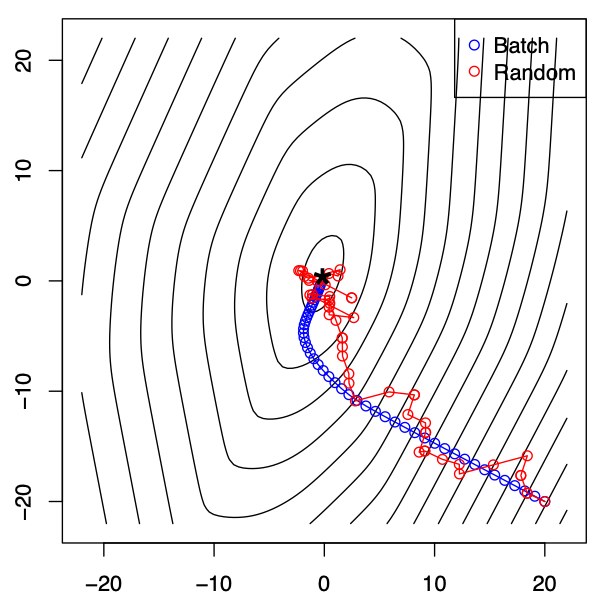
\includegraphics[height=0.6\textheight]{figures/batch-vs-stochastic.png}
    \end{figure}
    \end{column}
    \begin{column}{0.6\textwidth}
        Rule of thumb for stochastic methods:
        \begin{itemize}
            \item Stochastic methods work well far from the optimum
            \item But struggle close the the optimum
        \end{itemize}
    \end{column}
    \end{columns}
    (Slide adapted from Ryan Tibshirani)
\end{frame}

%\begin{frame}{Minibatch Gradient}
%\begin{itemize}
%\item Is the minibatch gradient random?
%\pause
%\item What's its expectation?
%\item What's the expected value of the \textbf{minibatch gradient}?
%\begin{eqnarray*}
%\ex\left[\del\hat{R}_{N}(w)\right] & = & \frac{1}{N}\sum_{i=1}^{N}\ex\left[\del_{w}\ell(f_{w}(x_{m_{i}}),y_{m_{i}})\right]\\
%& = & \ex\left[\del_{w}\ell(f_{w}(x_{m_{1}}),y_{m_{1}})\right]\\
%& = & \sum_{i=1}^{n}\pr\left(m_{1}=i\right)\del_{w}\ell(f_{w}(x_{i}),y_{i})\\
%& = & \frac{1}{n}\sum_{i=1}^{n}\del_{w}\ell(f_{w}(x_{i}),y_{i})\\
%& = & \del\hat{R}_{n}(w)
%\end{eqnarray*}
%\end{itemize}

%\begin{itemize}
%\item \emph{Technical note:} We only assumed that each point in the minibatch
%is equally likely to be any of the $n$ points in the batch -- no
%independence needed. So still true if we're sampling without replacement.
%Still true if we sample one point randomly and reuse it $N$ times.
%\end{itemize}
%\end{frame}
%
\begin{frame}{Minibatch Gradient Properties}
\begin{itemize}
\item The minibatch gradient is an \textbf{unbiased estimator} for the {[}full{]}
batch gradient. What does that mean?
\pause
\[
\ex\left[\del\hat{R}_{N}(w)\right]=\del\hat{R}_{n}(w)
\]
\pause
\item The bigger the minibatch, the better the estimate. 
    $$
        \frac{1}{N}\text{Var}\pb{\del\hat{R}_1(w)} = 
        \text{Var}\pb{\del\hat{R}_N(w)}
        $$
\pause
\item Tradeoffs of minibatch size:
\begin{itemize}
\item Bigger $N$ $\implies$Better estimate of gradient, but slower (more
data to process)
\item Smaller $N$ $\implies$Worse estimate of gradient, but can be quite
fast 
\end{itemize}
\pause
\item Because of vectorization, we can often get minibatches of certain sizes for free
\end{itemize}
\end{frame}
%
\begin{frame}
    {Convergence of SGD}
    \begin{itemize}
        \item For convergence guarantee, use \textbf{diminishing step sizes},
            e.g. $\eta_k = 1/k$
        \item Theoretically, GD is much faster than SGD in terms of convergence rate:
            \begin{itemize}
                \item much faster to add a digit of accuracy.
                \item but most of that advantage comes into play once we're already pretty close to the minimum.
                \item However, in many ML problems we don't care about optimizing to high accuracy
            \end{itemize}
    \end{itemize}
\end{frame}
%
\begin{frame}{Step Sizes in Minibatch Gradient Descent}
\begin{block}{Minibatch Gradient Descent (minibatch size $N$)}
\begin{itemize}
\item initialize $w=0$
\item repeat
\begin{itemize}
\item randomly choose $N$ points $\left\{ (x_{i},y_{i})\right\} _{i=1}^{N}\subset\cd_{n}$
\item $w\gets w-\eta\left[\frac{1}{N}\sum_{i=1}^{N}\del_{w}\ell(f_{w}(x_{i}),y_{i})\right]$
\end{itemize}
\end{itemize}
\end{block}

    \begin{itemize}
        \item For SGD, fixed step size can work well in practice.
        \item Typical approach: Fixed step size reduced by constant factor
whenever validation performance stops improving. 
\item Other tricks: Bottou (2012), ``Stochastic gradient descent tricks''
    \end{itemize}
\end{frame}
%
\begin{frame}{Summary}
\begin{itemize}
\item \textbf{Gradient descent} or \textbf{``full-batch'' gradient descent}
\begin{itemize}
\item Use full data set of size $n$ to determine step direction
\end{itemize}

\item \textbf{Minibatch gradient descent}
\begin{itemize}
    \item Use a \textbf{random} subset of size $N$ to determine step direction

%\item Yoshua Bengio says\footnote{See Yoshua Bengio's ``Practical recommendations for gradient-based
%training of deep architectures'' \url{http://arxiv.org/abs/1206.5533}.}:
%\begin{itemize}
%\item $N$ is typically between $1$ and few hundred
%\item $N=32$ is a good default value
%\item With $N\ge10$ we get computational speedup (per datum touched)
%\end{itemize}
\end{itemize}

\item \textbf{Stochastic gradient descent}
\begin{itemize}
\item Minibatch with $N=1$.
\item Use a single randomly chosen point to determine step direction.
\end{itemize}
\end{itemize}

    These days terminology isn't used so consistently, so always clarify
    the {[}mini{]}batch size.

    SGD is much more efficient in time and memory cost and has been quite successful in large-scale ML.
\end{frame}

\begin{frame}
    {Example: Logistic regression with $\ell_2$ regularization}
        Batch methods converge faster :
    \begin{figure}
        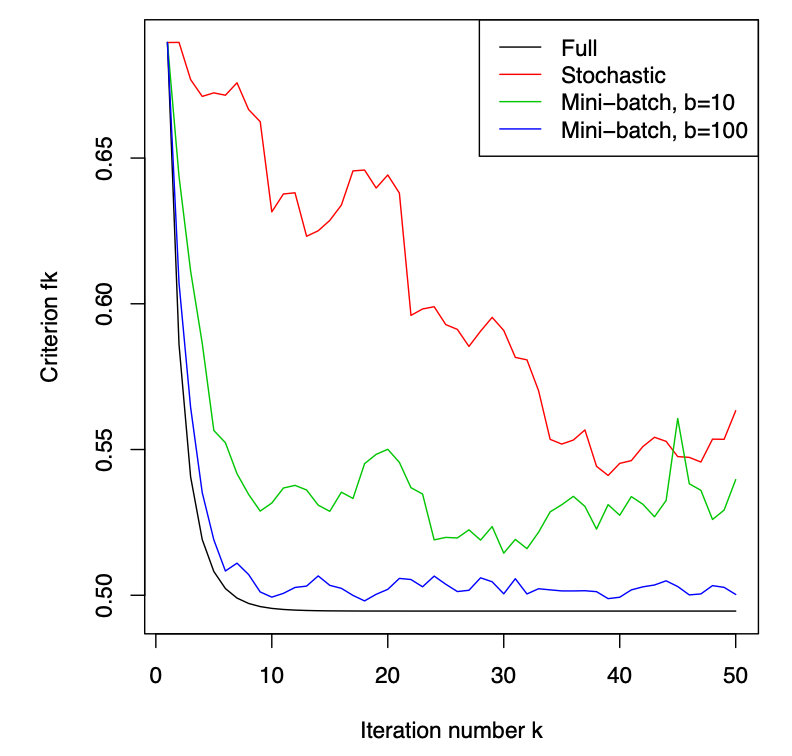
\includegraphics[height=0.7\textheight]{figures/logistic-sgd-loss}
    \end{figure}
    \vspace{-2em}
    (Example from Ryan Tibshirani)
\end{frame}

\begin{frame}
    {Example: Logistic regression with $\ell_2$ regularization}
        Stochastic methods are computationally more efficient:
    \begin{figure}
        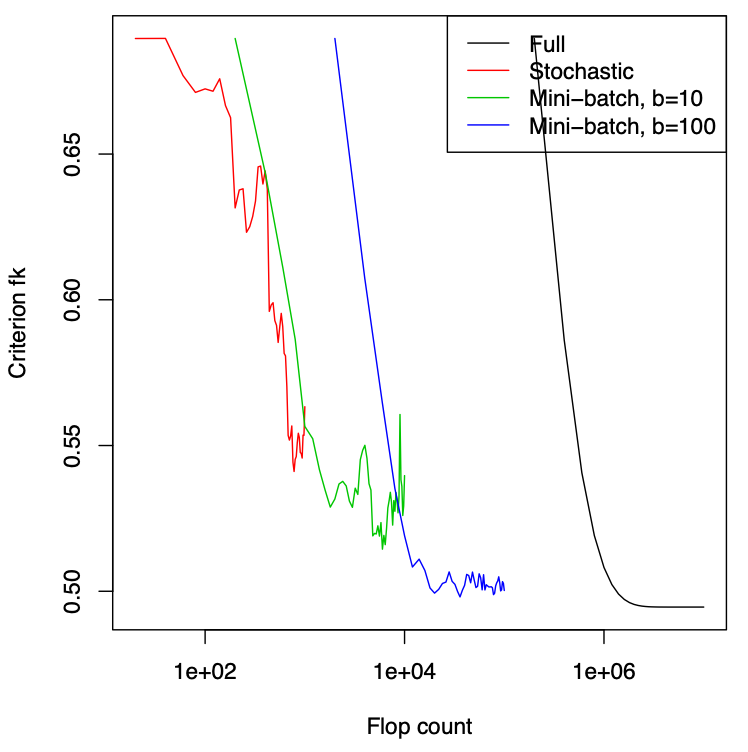
\includegraphics[height=0.7\textheight]{figures/logistic-sgd-flop}
    \end{figure}
    \vspace{-2em}
    (Example from Ryan Tibshirani)
\end{frame}

\begin{frame}
    {Example: Logistic regression with $\ell_2$ regularization}
        Batch methods are much faster close to the optimum:
    \begin{figure}
        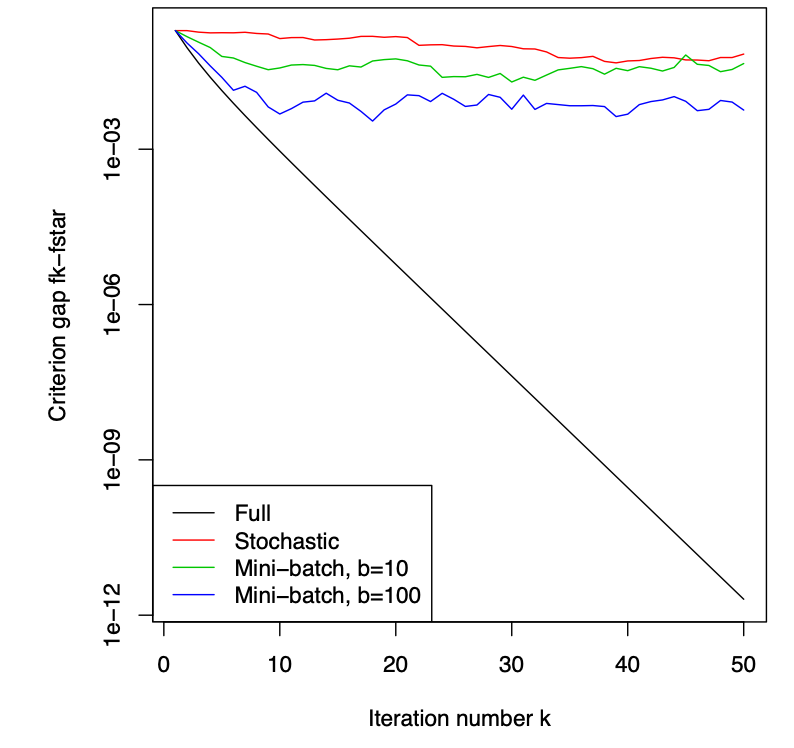
\includegraphics[height=0.7\textheight]{figures/logistic-sgd-optimality}
    \end{figure}
    \vspace{-2em}
    (Example from Ryan Tibshirani)
\end{frame}

\section{Loss Functions: Regression}
\begin{frame}{Regression Problems}
\begin{itemize}
    \item Examples:
        \begin{itemize}
            \item Predicting the stock price given history prices
            \item Predicting medical cost of given age, sex, region, BMI etc.
            \item Predicting the age of a person based on their photos
        \end{itemize}

        \pause
\item Spaces:
\begin{itemize}
\item Input space $\cx=\reals^{d}$
\item Action space $\ca=\reals$
\item Outcome space $\cy=\reals$.
\end{itemize}
\pause
\item Notation:
\begin{itemize}
\item $\hat{y}$ is the predicted value (the action)
\item $y$ is the actual observed value (the outcome)
\end{itemize}
\end{itemize}
\end{frame}
%
\begin{frame}{Loss Functions for Regression}

\begin{itemize}
\item A loss function in general:
\[
\left(\hat{y},y\right)\mapsto\ell(\hat{y},y)\in\reals
\]

\pause
\item Regression losses usually only depend on the \textbf{residual $r=y-\hat{y}$.}

\begin{itemize}
\item what you have to add to your prediction to get the correct answer.
\end{itemize}

\pause
\item A loss $\ell(\hat{y},y)$ is called \textbf{distance-based }if:
\begin{enumerate}
\item It only depends on the residual: 
\[
\ell(\hat{y},y)=\psi(y-\hat{y})\quad\text{for some \ensuremath{\psi}:\ensuremath{\reals\to\reals}}
\]


\item It is zero when the residual is $0$: 
\[
\psi(0)=0
\]
\end{enumerate}
\end{itemize}
\end{frame}
%
\begin{frame}{Distance-Based Losses are Translation Invariant}
\begin{itemize}
\item Distance-based losses are translation-invariant. That is,
\[
\ell(\hat{y}+b,y+b)=\ell\left(\hat{y},y\right)\qquad\forall b\in\reals.
\]

\item When might you not want to use a translation-invariant loss?

\pause{}
\item Sometimes the relative error $\frac{\hat{y}-y}{y}$ is a more natural
loss (but not translation-invariant)

\pause
\item Often you can transform response $y$ so it's translation-invariant
(e.g. log transform)
\end{itemize}

\end{frame}

\begin{frame}{Some Losses for Regression}
\begin{itemize}
\item \textbf{Residual: $r=y-\hat{y}$}
\item \textbf{Square} or $\ell_{2}$ Loss: $\ell(r)=r^{2}$ 
\pause
\item \textbf{Absolute} or \textbf{Laplace} or $\ell_{1}$ Loss: $\ell(r)=\left|r\right|$ 
\pause
\end{itemize}

\begin{description}
\item [{%
\begin{tabular}{|c|c|c|c|}
\hline 
$y$ & $\hat{y}$ & $\left|r\right|=\left|y-\hat{y}\right|$ & $r^{2}=\left(y-\hat{y}\right)^{2}$\tabularnewline
\hline 
\hline 
1 & 0 & 1 & 1\tabularnewline
\hline 
5 & 0 & 5 & 25\tabularnewline
\hline 
10 & 0 & 10 & 100\tabularnewline
\hline 
50 & 0 & 50 & 2500\tabularnewline
\hline 
\end{tabular}}]~
\end{description}

\begin{itemize}
    \item Outliers typically have large residuals. (What is an outlier?)
\item Square loss much more affected by outliers than absolute loss.
\end{itemize}
\end{frame}

\begin{frame}{Loss Function Robustness}
\begin{itemize}
\item \textbf{Robustness }refers to how affected a learning algorithm is
by outliers.
\end{itemize}
\begin{center}
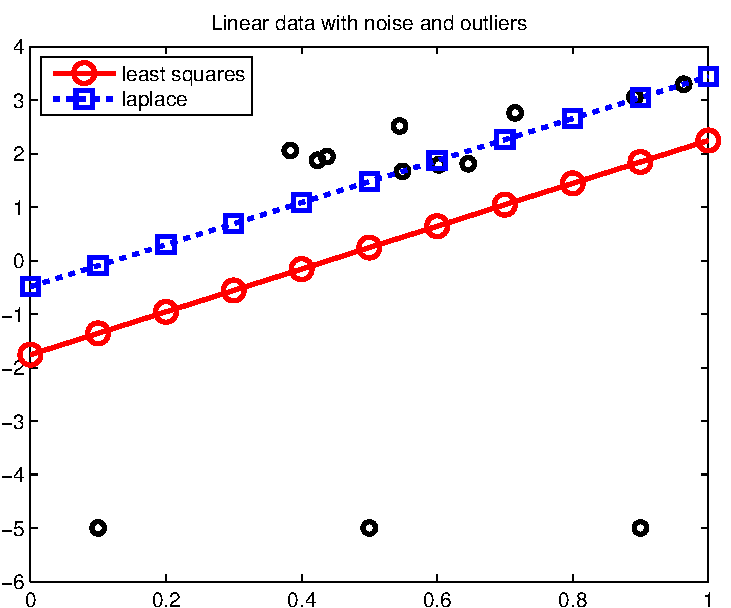
\includegraphics[height=0.6\textheight]{figures/fig7.6a}\let\thefootnote\relax\footnotetext{\tiny{KPM Figure 7.6}}
\par\end{center}

\end{frame}

\begin{frame}{Some Losses for Regression}

\let\thefootnote\relax\footnotetext{\tiny{KPM Figure 7.6}}
\begin{itemize}
\item \textbf{Square} or $\ell_{2}$ Loss: $\ell(r)=r^{2}$ (\emph{not robust})

\item \textbf{Absolute} or \textbf{Laplace} Loss: $\ell(r)=\left|r\right|$
(\emph{not differentiable})
\begin{itemize}
\item gives \textbf{median regression}
\end{itemize}

\item \textbf{Huber} Loss: Quadratic for $\left|r\right|\le\delta$ and
linear for $\left|r\right|>\delta$ (\emph{robust and differentiable})
    \begin{itemize}
    \item Equal values and slopes at $r=\delta$ 
    \end{itemize}
\end{itemize}
\begin{center}
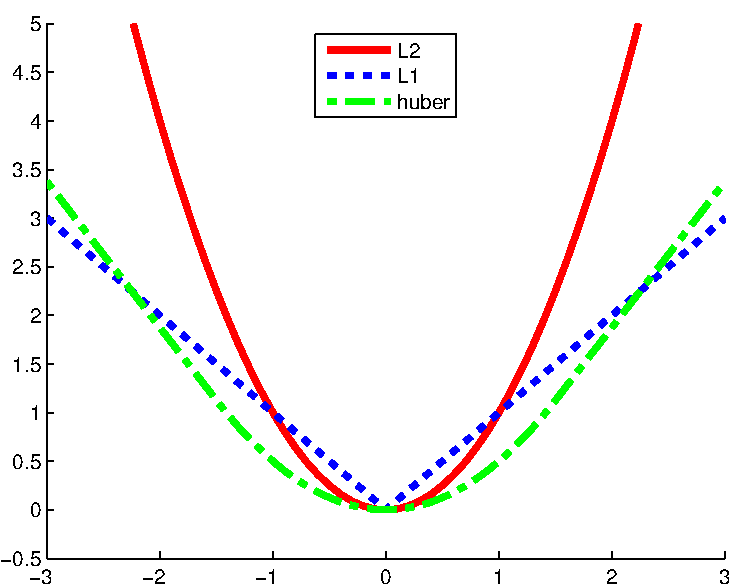
\includegraphics[height=0.4\textheight]{figures/fig7.6b}
\par\end{center}

\end{frame}


\section{Classification Loss Functions}

\begin{frame}{The Classification Problem}
    \begin{itemize}
    \item Examples:
        \begin{itemize}
            \item Predict whether the image contains a cat
            \item Predict whether the email is SPAM
        \end{itemize}

    \pause

    \item Classification spaces:
    \begin{itemize}
        \item Input space $\reals^d$
        \item Outcome space $\cy=\left\{ -1,1\right\} $
        \item Action space $\ca=\reals$ (easier to work with than $\ca=\left\{ -1,1\right\} $)
    \end{itemize}

            \pause
    \item Inference:
        \vspace{-2ex}
        \begin{itemize}
            \item[]
            \begin{align*}
            f(x)>0\;\implies & \mbox{Predict }1\\
            f(x)<0\;\implies & \mbox{Predict }-1
            \end{align*}
        \end{itemize}
    \end{itemize}
\end{frame}

\begin{frame}{The Score Function}
\begin{itemize}
\item Action space $\ca=\reals\qquad$ Output space $\cy=\left\{ -1,1\right\} $
\item \textbf{Real-valued prediction function} $f:\cx\to\reals$
\end{itemize}

\begin{definition}
The value $f(x)$ is called the \textbf{score} for the input $x$. 
\end{definition}

\begin{itemize}
\item In this context, $f$ may be called a \textbf{score function}.
\item The magnitude of the score can be interpreted as our \textbf{confidence
of our prediction}.
\end{itemize}
\end{frame}
%
\begin{frame}{The Margin}
\begin{definition}
The \textbf{margin} (or \textbf{functional margin})\textbf{ }for a predicted
score $\hat{y}$ and the true class $y\in\left\{ -1,1\right\} $ is $y\hat{y}$. 
\end{definition}

\pause
\begin{itemize}
\item The margin is often written as $yf(x)$, where $f(x)$ is our score function.

\item The margin is a measure of how \textbf{correct} we are:

\begin{itemize}
\item If $y$ and $\hat{y}$ are the same sign, prediction is \textbf{correct}
and margin is \textbf{positive}.
\item If $y$ and $\hat{y}$ have different sign, prediction is \textbf{incorrect}
and margin is \textbf{negative}.
\end{itemize}
    \item We want to \textbf{maximize the margin}
    \item Most classification losses depend only on the margin (they are \textbf{margin-based losses}).
\end{itemize}
\end{frame}
%

\begin{frame}{Classification Losses: $0-1$ Loss}
\begin{itemize}
    \item If $\tilde{f}$ is the inference function ($1$ if $f(x) > 0$ and $-1$ otherwise), then
    \item The \textbf{0-1 loss} for $f:\cx\to\left\{ -1,1\right\} $:
    \[
        \loss\left(f(x),y\right)=\ind{\tilde{f}(x)\neq y}
    \]
\item Empirical risk for $0-1$ loss:
\[
\hat{R}_{n}(f)=\frac{1}{n}\sum_{i=1}^{n}\ind{y_{i}f(x_{i})\leq0}
\]
\end{itemize}

\begin{alertblock}{Minimizing empirical $0-1$ risk not computationally feasible}

$\hat{R}_{n}(f)$ is non-convex, not differentiable (in fact, discontinuous!). 

Optimization is \textbf{NP-Hard}.
\end{alertblock}
\end{frame}

\begin{frame}{Classification Losses}

Zero-One loss: $\loss_{\text{0-1}}=\ind{m\le0}$
\begin{center}
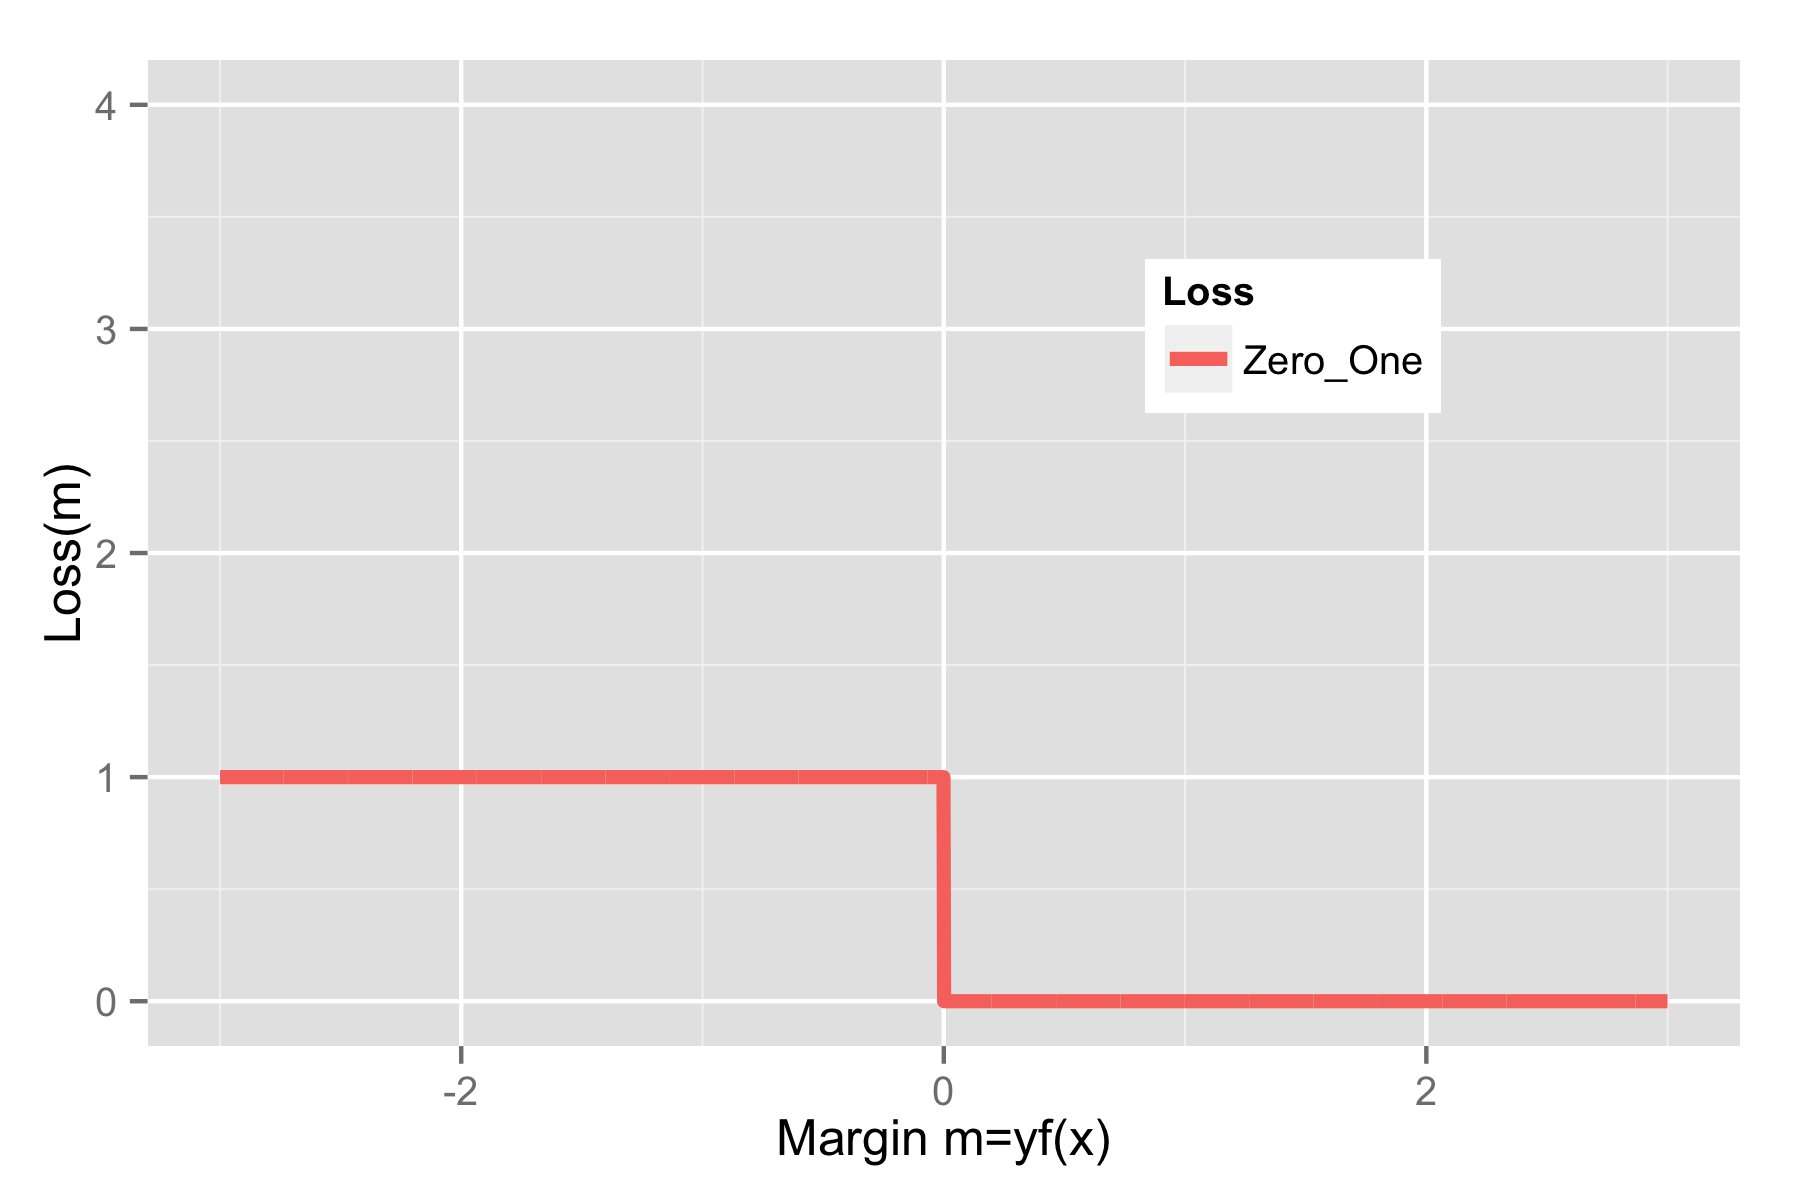
\includegraphics[height=0.6\textheight]{figures/loss.Zero_One}
\par\end{center}
\begin{itemize}
\item x-axis is \textbf{margin}: $m>0\iff\text{correct classification}$
\end{itemize}

\end{frame}

\begin{frame}{Classification Losses}

SVM/Hinge loss: $\loss_{\text{Hinge}}=\max\left(1-m,0\right)$
\begin{center}
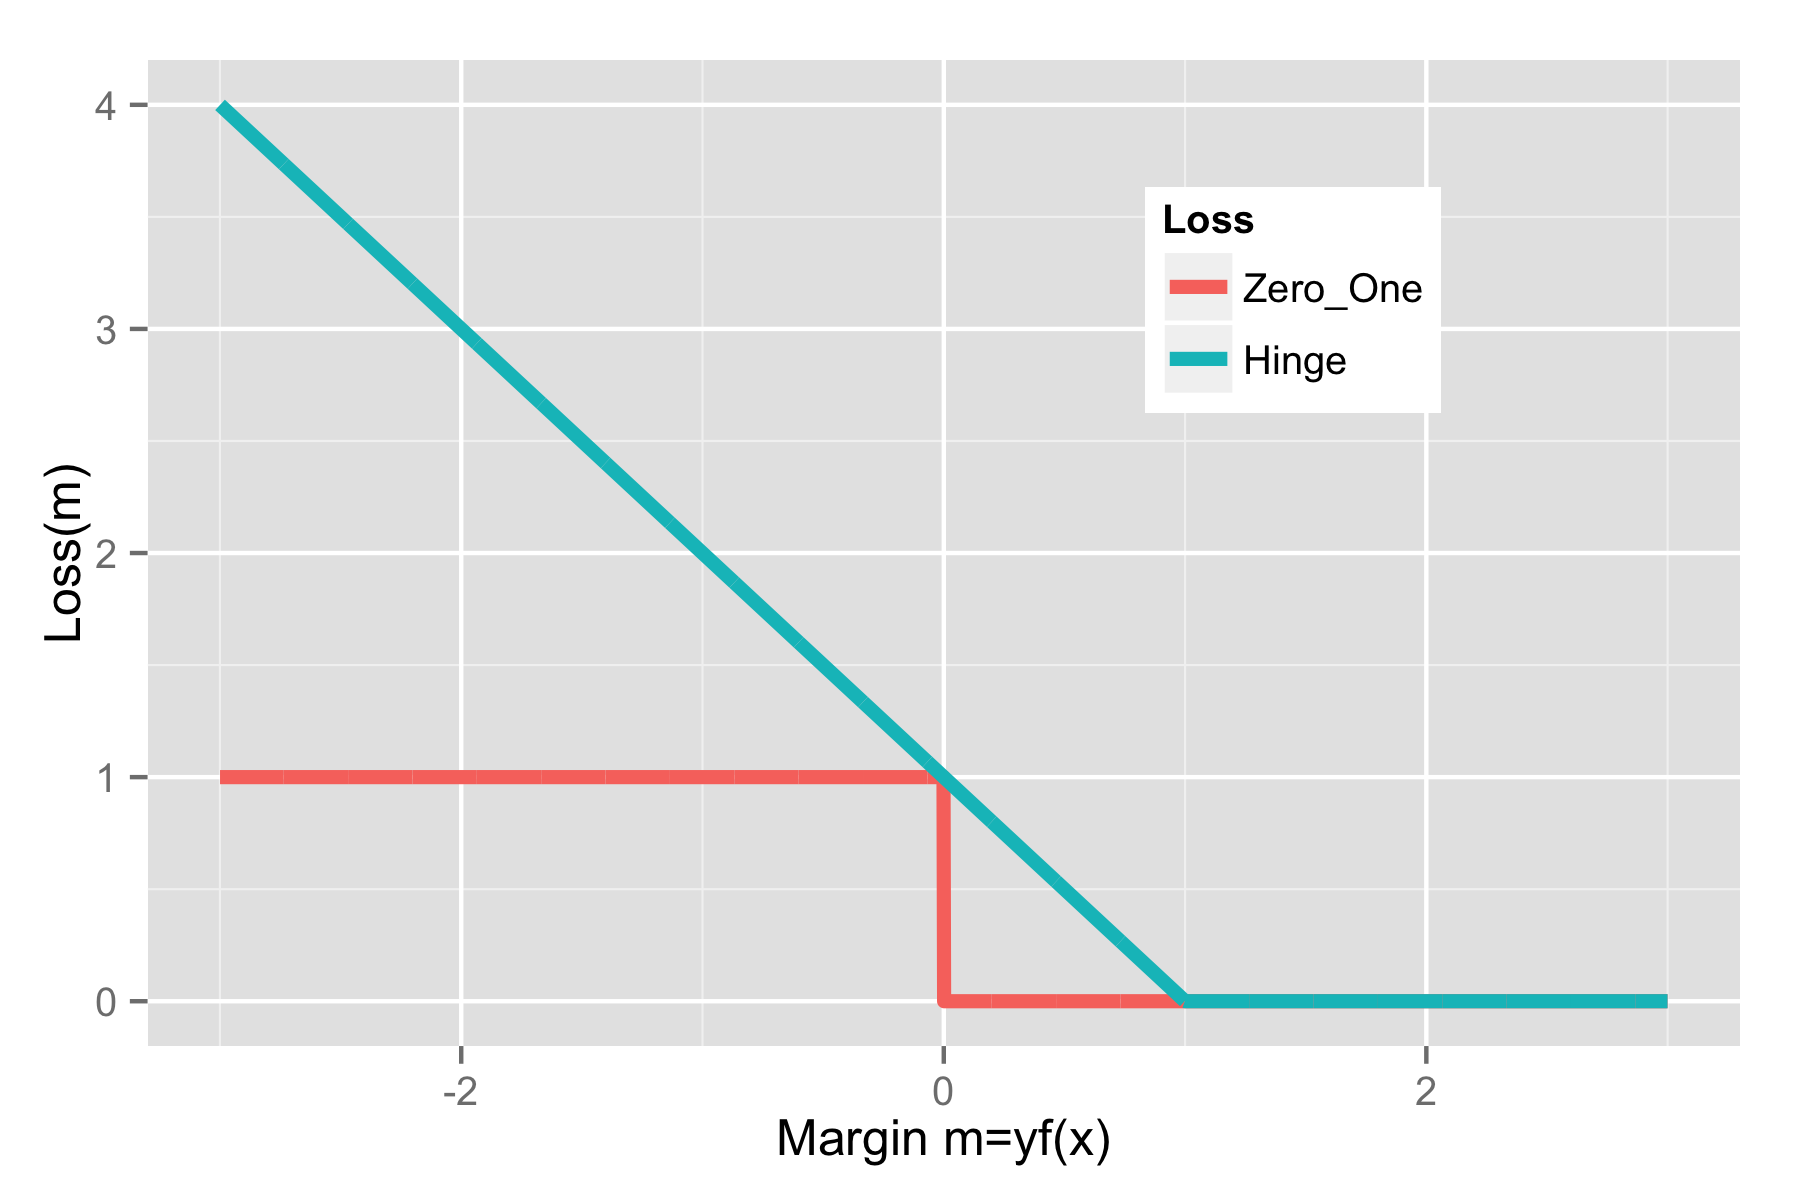
\includegraphics[height=0.6\textheight]{figures/loss.Zero_One.Hinge}
\par\end{center}

Hinge is a \textbf{convex}, \textbf{upper bound} on $0-1$ loss. Not
differentiable at $m=1$.
%We have a \textbf{``margin error''} when $m<1$.
\end{frame}

\begin{frame}{Classification Losses}

Logistic/Log loss: $\loss_{\text{Logistic}}=\log\left(1+e^{-m}\right)$
\begin{center}
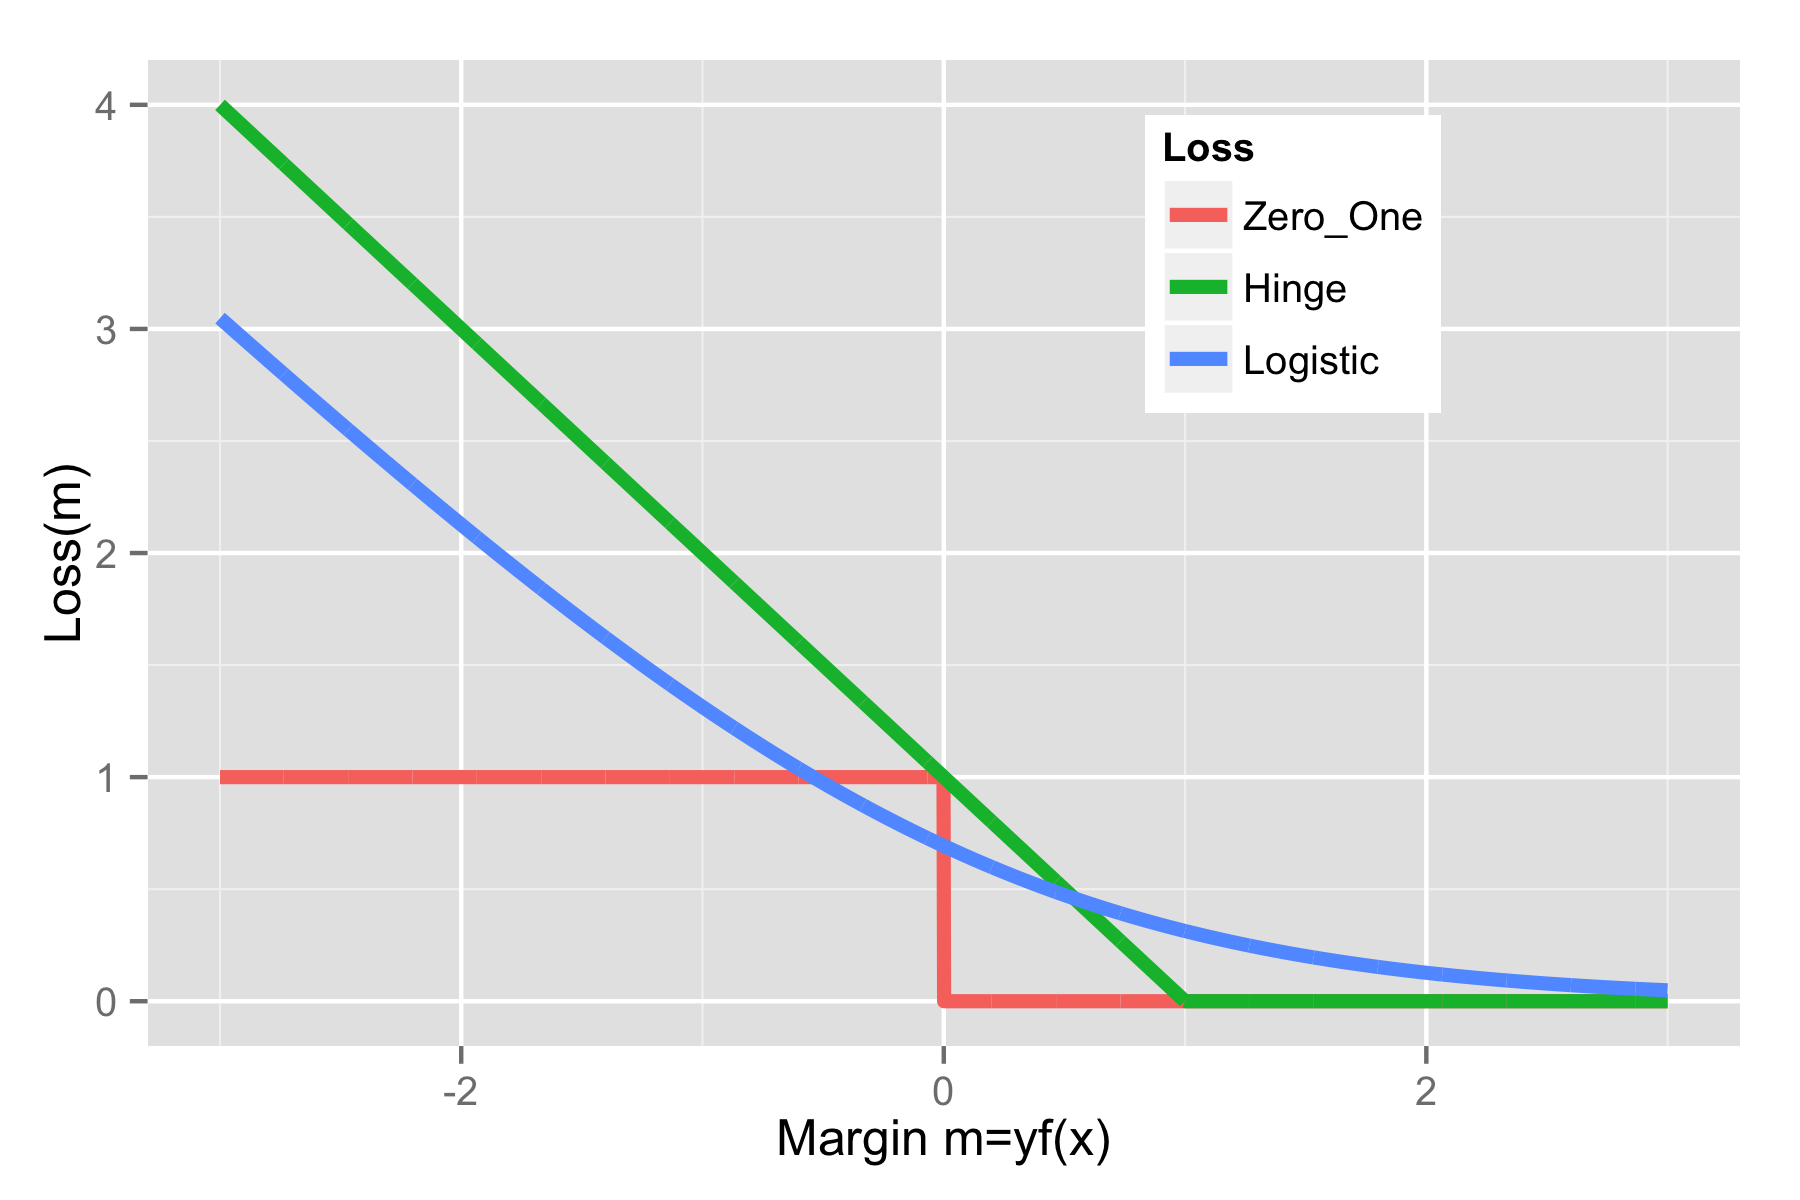
\includegraphics[height=0.6\textheight]{figures/loss.Zero_One.Hinge.Logistic}
\par\end{center}

Logistic loss is differentiable. Logistic loss always rewards a larger margin
(the loss is never 0).
\end{frame}

\begin{frame}{What About Square Loss for Classification?}
\begin{itemize}
\item Action space $\ca=\reals\qquad$Output space $\cy=\left\{ -1,1\right\} $
\item Loss $\ell(f(x),y)=\left(f(x)-y\right)^{2}$.

\item Turns out, can write this in terms of margin $m=f(x)y$:
\begin{eqnarray*}
\ell(f(x),y) & = & \left(f(x)-y\right)^{2}=\left(1-f(x)y\right)^{2}=\left(1-m\right)^{2}
\end{eqnarray*}
\item Prove using fact that $y^{2}=1$, since $y\in\left\{ -1,1\right\} $.
\end{itemize}
\end{frame}

\begin{frame}{What About Square Loss for Classification?}
\begin{center}
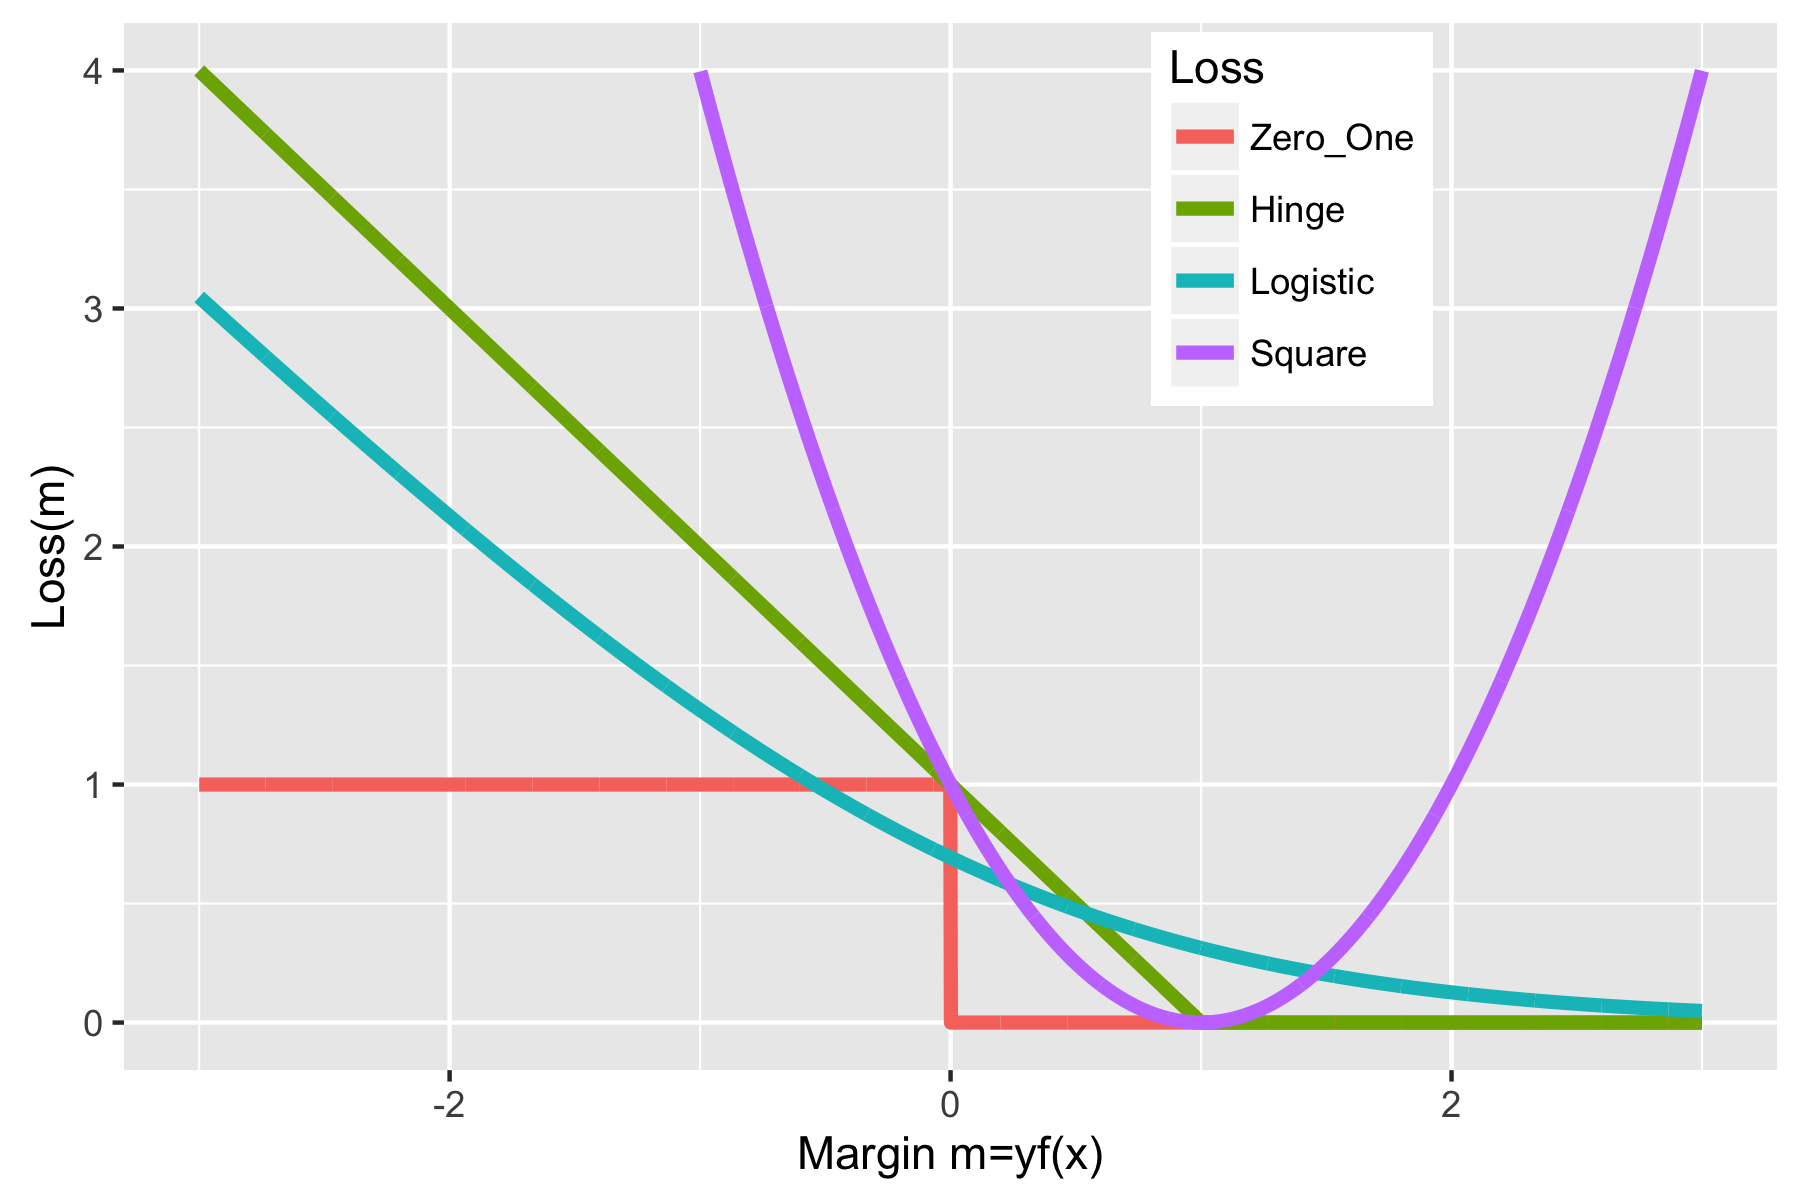
\includegraphics[height=0.6\textheight]{figures/loss.Zero_One.Hinge.Logistic.Square}
\par\end{center}

Heavily penalizes outliers (e.g. mislabeled examples).

May have higher sample complexity (i.e. needs more data) than hinge
\& logistic\footnote{{\tiny{}Rosasco et al's ``Are Loss Functions All the Same?'' \url{http://web.mit.edu/lrosasco/www/publications/loss.pdf}}}. 

\end{frame}


\end{document}
